%%% License: Creative Commons Attribution Share Alike 4.0 (see https://creativecommons.org/licenses/by-sa/4.0/)


%%%%%%%%%%%%%%%%%%%%%%%%%%%%%%%%%%%%%%%%%

%----------------------------------------------------------------------------------------
%	PACKAGES AND OTHER DOCUMENT CONFIGURATIONS
%----------------------------------------------------------------------------------------

\documentclass[a4paper]{article}

\usepackage{amssymb}
\usepackage{enumerate}
\usepackage[usenames,dvipsnames]{color}
\usepackage{fancyhdr} % Required for custom headers
\usepackage{lastpage} % Required to determine the last page for the footer
\usepackage{extramarks} % Required for headers and footers
\usepackage[usenames,dvipsnames]{color} % Required for custom colors
\usepackage{graphicx} % Required to insert images
\usepackage{listings} % Required for insertion of code
\usepackage{courier} % Required for the courier font
\usepackage[table]{xcolor}
\usepackage{amsfonts,amsmath,amsthm,parskip,setspace,url}
\usepackage[section]{placeins}
\usepackage[a4paper]{geometry}
\usepackage[USenglish]{babel}
\usepackage[utf8]{inputenc}
\usepackage{tikz}


% Margins
\topmargin=-0.45in
\evensidemargin=0in
\oddsidemargin=0in
\textwidth=6.5in
\textheight=9.0in
\headsep=0.6in

\linespread{1.1} % Line spacing



%----------------------------------------------------------------------------------------
%   FORMATTING
%----------------------------------------------------------------------------------------
% Set up the header and footer
\pagestyle{fancy}
\lhead[c]{\textbf{{\color[rgb]{.5,0,0} K{\o}benhavns\\Universitet }}} % Top left header
\chead{\textbf{{\color[rgb]{.5,0,0} \Class }}\\ \hmwkTitle  } % Top center head
\rhead{\instructor \\ \theprofessor} % Top right header
\lfoot{\lastxmark} % Bottom left footer
\cfoot{} % Bottom center footer
\rfoot{Page\ \thepage\ of\ \protect\pageref{LastPage}} % Bottom right footer
\renewcommand\headrulewidth{0.4pt} % Size of the header rule
\renewcommand\footrulewidth{0.4pt} % Size of the footer rule


% Other formatting stuff
%\setlength\parindent{12pt}
\setlength{\parskip}{5 pt}
%\theoremstyle{definition} \newtheorem{ex}{\textbf{\Large{Exercise & #}\\}}
\usepackage{titlesec}
\titleformat{\section}[hang]{\normalfont\bfseries\Large}{Problem \thesection:}{0.5em}{}




%----------------------------------------------------------------------------------------
%	NAME AND CLASS SECTION
%----------------------------------------------------------------------------------------
\newcommand{\hmwkTitle}{Exercises for Lecture 4} % Assignment title
\newcommand{\Class}{Mechanism Design} % Course/class
\newcommand{\instructor}{Fall 2023} % TA
\newcommand{\theprofessor}{Prof. Egor Starkov} % Professor




%----------------------------------------------------------------------------------------
%   SOLUTIONS
%----------------------------------------------------------------------------------------
\newif\ifsolutions
\solutionstrue




\begin{document}

\begin{center}
		\LARGE\textbf{Exercises for Lecture 4:\\ Revenue equivalence}
\end{center}


\section{Payoff equivalence in BIC mechanisms}

	Prove the payoff equivalence result for BIC mechanisms using the analog of the argument we had for DSIC mechanisms (i.e., by showing monotonicity first). Assume that players' types are mutually independent.
	
\ifsolutions
\section*{Solution}

	BIC IC constraints for types $\theta_i$ and $\hat{\theta}_i$ to not be willing to mimic each other are:
	\begin{align}
		\mathbb{E}_{\theta_{-i}}\left[ \theta_{i} k(\theta_i,\theta_{-i}) - t(\theta_i,\theta_{-i}) \right] &\geq 
		\mathbb{E}_{\theta_{-i}}\left[ \theta_{i} k(\hat{\theta}_i,\theta_{-i}) - t(\hat{\theta}_i,\theta_{-i}) \right],
		\label{eq:IC1}
		\\
		\mathbb{E}_{\theta_{-i}}\left[ \hat{\theta}_{i} k(\theta_i,\theta_{-i}) - t(\theta_i,\theta_{-i}) \right] &\leq 
		\mathbb{E}_{\theta_{-i}}\left[ \hat{\theta}_{i} k(\hat{\theta}_i,\theta_{-i}) - t(\hat{\theta}_i,\theta_{-i}) \right].
		\label{eq:IC2}
	\end{align}
	Add and subtract $\hat{\theta}_{i} k(\hat{\theta}_i,\theta_{-i})$ from the right-hand side of \eqref{eq:IC1} to obtain
	\begin{align}
		\bar{U}_i(\theta_i) \geq \bar{U}_i(\hat{\theta}_i) + (\theta_i - \hat{\theta}_i) \mathbb{E}_{\theta_{-i}}\left[ k(\hat{\theta}_i,\theta_{-i}) \right], \label{eq:IC1b}
	\end{align}
	where $\bar{U}_i(\theta_i)$ is the interim expected utility of type $\theta_i$ from truthtelling: $\bar{U}_i(\theta_i) \equiv \mathbb{E}_{\theta_{-i}}\left[ \theta_{i} k(\theta_i,\theta_{-i}) - t(\theta_i,\theta_{-i}) \right] = \mathbb{E}_{\theta_{-i}}\left[ U(\theta_i,\theta_{-i}) \right]$.
	Doing an analogous manipulation with \eqref{eq:IC2}, combining the resulting inequality with \eqref{eq:IC1b}, and rearranging the two then yields the following, under the assumption that $\theta_i > \hat{\theta}_i$ (you can do the same with the converse):
	\begin{align}
		\mathbb{E}_{\theta_{-i}}\left[ k(\theta_i,\theta_{-i}) \right] \geq \frac{\bar{U}_i(\theta_i) - \bar{U}_i(\hat{\theta}_i)}{\theta_i - \hat{\theta}_i} \geq \mathbb{E}_{\theta_{-i}}\left[ k(\hat{\theta}_i,\theta_{-i}) \right] .
		\label{eq:ICsandwich}
	\end{align}
	The expected allocation $\bar{k}_i(\theta_i) \equiv \mathbb{E}_{\theta_{-i}}\left[ k(\theta_i,\theta_{-i}) \right]$ is thus monotone in $\theta_i$. Monotonicity implies continuity almost everywhere, hence the following is true for almost all $\theta_i$:
	\begin{align}
		\lim_{\hat{\theta}_i \to \theta_i} \bar{k}_i(\hat{\theta}_i) = \bar{k}_i(\theta_i).
		\label{eq:Klimit}
	\end{align}
	Now take limits of \eqref{eq:ICsandwich} as $\hat{\theta}_i \to \theta_i$. By the theorem about two policemen\footnote{\url{https://en.wikipedia.org/wiki/Squeeze_theorem}} together with \eqref{eq:Klimit}, we have that
	\begin{align}
		\lim_{\hat{\theta}_i \to \theta_i} \frac{\bar{U}_i(\theta_i) - \bar{U}_i(\hat{\theta}_i)}{\theta_i - \hat{\theta}_i} = \bar{k}_i(\theta_i)
		\label{eq:derivlimit}
	\end{align}
	for almost all $\theta_i$.
	The left-hand side of \eqref{eq:derivlimit} is the definition of the derivative of $\bar{U}_i$, hence $\frac{d\bar{U}_i(\theta_i)}{d \theta_i}$ exists and $\frac{d\bar{U}_i(\theta_i)}{d \theta_i} = \bar{k}_i(\theta_i)$ almost everywhere.\footnote{At points of discontinuity of $\bar{k}_i(\theta_i)$, function $\bar{U}_i(\theta_i)$ will have a kink, and all values between the two limits $\lim_{\hat{\theta}_i \nearrow \theta_i} \bar{k}_i(\hat{\theta}_i)$ and $\lim_{\hat{\theta}_i \searrow \theta_i} \bar{k}_i(\hat{\theta}_i)$ will be subderivatives of $\bar{U}_i$ at that point. For purposes of applying the Fundamental theorem of calculus, we can safely take $\bar{k}_i(\theta_i)$ to mean the derivative of $\bar{U}_i$ at such points.}
	Applying the Fundamental theorem of calculus, we get that for any $\hat{\theta}_i$, the following holds:
	\begin{align}
		\bar{U}_i(\theta_i) &= \bar{U}_i(\hat{\theta}_i) + \int_{\hat{\theta}_i}^{\theta_i} \bar{k}_i(s) ds
		\\
		&= \bar{U}_i(\hat{\theta}_i) + \int_{\hat{\theta}_i}^{\theta_i} \mathbb{E}_{\theta_{-i}}\left[ k(s,\theta_{-i}) \right] ds.
	\end{align}
	We have obtained the envelope representation of payoffs, and now we can make the final step towards the revenue equivalence. Recall that
	\begin{align*}
		\bar{U}_i(\theta_i) &= \mathbb{E}_{\theta_{-i}}\left[ \theta_{i} k(\theta_i,\theta_{-i}) - t(\theta_i,\theta_{-i}) \right]
		\\ \Leftrightarrow
		\mathbb{E}_{\theta_{-i}}\left[ t(\theta_i,\theta_{-i}) \right] &= -\bar{U}_i(\theta_i) + \mathbb{E}_{\theta_{-i}}\left[ \theta_{i} k(\theta_i,\theta_{-i}) \right] 
		\\
		&= -\bar{U}_i(\hat{\theta}_i) - \int_{\hat{\theta}_i}^{\theta_i} \mathbb{E}_{\theta_{-i}}\left[ k(s,\theta_{-i}) \right] ds + \mathbb{E}_{\theta_{-i}}\left[ \theta_{i} k(\theta_i,\theta_{-i}) \right] .
	\end{align*}
	Therefore, for any two BIC DRMs $x=(k,t)$ and $x'=(k',t')$, if $\mathbb{E}_{\theta_{-i}}\left[ \theta_{i} k(\theta_i,\theta_{-i}) \right] = \mathbb{E}_{\theta_{-i}}\left[ \theta_{i} k'(\theta_i,\theta_{-i}) \right]$, then 
	\begin{align*}
		\mathbb{E}_{\theta_{-i}}\left[ t(\theta_i,\theta_{-i}) \right] - \mathbb{E}_{\theta_{-i}}\left[ t'(\theta_i,\theta_{-i}) \right]
		=
		-\bar{U}_i(\hat{\theta}_i) + \bar{U}'_i(\hat{\theta}_i),
	\end{align*}
	where on the RHS we have the equilibrium (truthtelling) utilities of some fixed type $\hat{\theta}_i$ in the two mechanisms. Denoting this difference by $h_i$ proves the statement of revenue equivalence.\footnote{To clarify why exactly we can denote $h_i \equiv -\bar{U}_i(\hat{\theta}_i) + \bar{U}'_i(\hat{\theta}_i)$: note that once we fix some respective ``comparison types'' $\hat{\theta}_i$ for every player $i$, this expression only depends on the identity of player $i$, but not on their actual type $\theta_i$, and not on other players' reports $\theta_{-i}$.}
\fi


\section{Efficient public good provision 2}

	Consider the public good provision problem from the previous problem set, described as follows.
	
	There is a society of $N$ people. They must collectively decide whether to implement a public project. Let $k \in \{0,1\}$ denote the outcome of this decision: $k=1$ if project is implemented, $k=0$ otherwise. Every person $i$ has some private valuation $\theta_i \in \mathbb{R}$ for the project, positive or negative. Preferences are linear, so $i$'s utility can be written as
	$$
		u_i(x,\theta) = \theta_i k(\theta) - t_i(\theta).
	$$
	Here $x=(k,t)$ stands for some direct mechanism which prescribes outcome $k(\theta) \in \{0,1\}$ and payment profile $t(\theta)$ given profile of reports $\theta$.
	
	\begin{enumerate}
		\item Fix an arbitrary $\theta_{-i}$ and suppose that we want to implement (in dominant strategies) an allocation rule that satisfies $k_i(\theta_i, \theta_{-i}) = \mathbb{I}\{\theta_i \geq \tilde{\theta}_i \}$ for some $\tilde{\theta}_i$ (where $\mathbb{I}\{\cdot\}$ is an indicator function).
		
		Use the envelope representation of payoffs to derive the (class of) transfer rule(s) for $i$ that DS-implements $k_i$ given $\theta_{-i}$.
		
		\item Suppose the public prject has cost $c > 0$. Find the efficient allocation rule $k^*(\theta)$. Use your findings from the previous question to derive the (class of) transfer rule(s) for all players that implements $k^*$ in dominant strategies.
		
		\item Conclude that \emph{only} Groves' transfers can DS-implement $k^*$ in this problem.
	\end{enumerate}

\ifsolutions
\section*{Solution}

\begin{enumerate}
	\item ERP (for DSIC mechanisms, since we are conditioning on $\theta_{-i}$ in this problem) tells us that the following \emph{must} hold in an IC mechanism:
	\begin{align*}
		U_i(\theta_i,\theta_{-i}) 
		&= U_i(\tilde{\theta}_i, \theta_{-i}) + \int\limits_{\tilde{\theta}_i}^{\theta_i} k_i(s,\theta_{-i}) ds
		\\
		&= U_i(\tilde{\theta}_i, \theta_{-i}) + \mathbb{I}\{\theta_i \geq \tilde{\theta}_i \} \cdot (\theta_i - \tilde{\theta}_i)
		\\
		&= U_i(\tilde{\theta}_i, \theta_{-i}) + (\theta_i - \tilde{\theta}_i)_+
	\end{align*}
	where we have chosen $\tilde{\theta}_i$ as our ``anchor'' type, and the second line used the allocation rule given in the problem. The third line above uses the simplifying notation $(x)_+ \equiv x \cdot \mathbb{I}\{x > 0\}$. Plugging $U_i(\theta_i,\theta_{-i}) = \theta_i k(\theta) - t_i(\theta)$, we get the expression for the transfers:
	\begin{align*}
		t_i(\theta_i, \theta_{-i}) 
		&= \theta_i k(\theta) - U_i(\tilde{\theta}_i, \theta_{-i}) - (\theta_i - \tilde{\theta}_i)_+
		\\
		&= \begin{cases}
			- U_i(\tilde{\theta}_i, \theta_{-i}) & \text{ if } \theta_i < \tilde{\theta}_i,
			\\
			\tilde{\theta}_i - U_i(\tilde{\theta}_i, \theta_{-i}) & \text{ if } \theta_i \geq \tilde{\theta}_i.
		\end{cases}
	\end{align*}
	Importantly, ERP implies that the transfer rule \emph{must} satisfy the form above to support the desired $k_i$ rule -- no other transfer rules would work.
	
	\item We can account for the cost by including it in the preferences of the principal: $u_0(x,\theta) = -c k + \sum_{i=1}^N t_i$. Then the efficient allocation rule is
	\begin{align*}
		k^*(\theta) 
		&\in \arg \max_{k \in \{0,1\}} \sum_{i=0}^N u_i((k,t),\theta)
		\\
		&\in \arg \max_{k \in \{0,1\}} \left\{\left(\sum_{i=1}^N \theta_i - c \right) k \right\}
		\\
		&= \mathbb{I} \left\{ \sum_{i=1}^N \theta_i > c \right\}.
	\end{align*}
	Note that it fits the representation given in the previous question, with $\tilde{\theta}_i \equiv c - \sum_{j\neq i} \theta_j$. Hence a transfer rule $t(\theta)$ DS-implements $k^*(\theta)$ if and only if it satisfies
	\begin{align} \label{eq:pubgood_groves}
		t_i(\theta_i, \theta_{-i}) 
		&= \begin{cases}
			h_i(\theta_{-i}) & \text{ if } \theta_i < \tilde{\theta}_i,
			\\
			c - \sum_{j\neq i} \theta_j + h_i(\theta_{-i}) & \text{ if } \theta_i \geq \tilde{\theta}_i,
		\end{cases}
	\end{align}
	where $h_i(\theta_{-i}) \equiv - U_i(\tilde{\theta}_i, \theta_{-i})$.
	
	\item It is easy to see that \eqref{eq:pubgood_groves} is exactly the expression for Groves' transfers in this problem, and ERP implies that in any DSIC mechanism with allocation rule $k^*$, the transfer rule \emph{must} satisfy \eqref{eq:pubgood_groves}. The statement in the question then follows.
\end{enumerate}
\fi 



\section{Implementation in auctions}

Consider the auction environment with two buyers and one item for sale. Suppose that each buyer $i$ has willingness to pay $\theta_i \in [0,1].$
\begin{enumerate}
	\item Draw a square with $\theta_1$ on the horizontal axis and $\theta_2$ on the vertical axis.  A point in the square
	represents a profile $(\theta_1, \theta_2)$.
	\item Draw a downward sloping curve through the box.
	\item Draw an upward sloping curve through the box that intersects the downward sloping curve (exactly once.)
	\item The region above your downward sloping curve is divided into two subregions by your upward sloping curve.  Label
	the subregion that is above your upward sloping curve with a $2$ and label the other subregion with a $1$.  Label
	the entire region that is below (and to the left of) your downward sloping curve with a $0$.
	\item Consider the allocation rule that is defined by your drawing.  In the $1$ region agent $1$ gets the
	good, in the $2$ region agent $2$ gets the good and in the $0$ region neither agent gets the good.  (On the boundary
	between regions pick the allocation from one of the neighboring regions. )  Find a transfer rule which, when
	coupled with your allocation rule, forms a DSIC mechanism.
	
	\emph{Hint: you will probably need to use the envelope representation of payoffs that we obtained when deriving payoff-equivalence:}
	\begin{equation*}
		U_i(\theta_i, \theta_{-i}) = U_i (\underline{\theta}_i,\theta_{-i}) + \int_{\underline{\theta}_i}^{\theta_i} k_i(s,\theta_{-i}) d s
	\end{equation*}
	\emph{In particular, you can derive transfers that support $k$ using the expression above. But if you did Problem 3 above, you already know that.}
	
	\item Is there any DSIC allocation rule that picks alternatives from the set $\{0,1,2\}$ that could not be represented by a drawing that follows the instructions given above?
	\\
	(If not: argue verbally why not. If yes: draw a graph and argue intuitively why the $k$ you drew would be DSIC.)
\end{enumerate}

\ifsolutions
\section*{Solution}

\begin{figure}
	\begin{center} 
		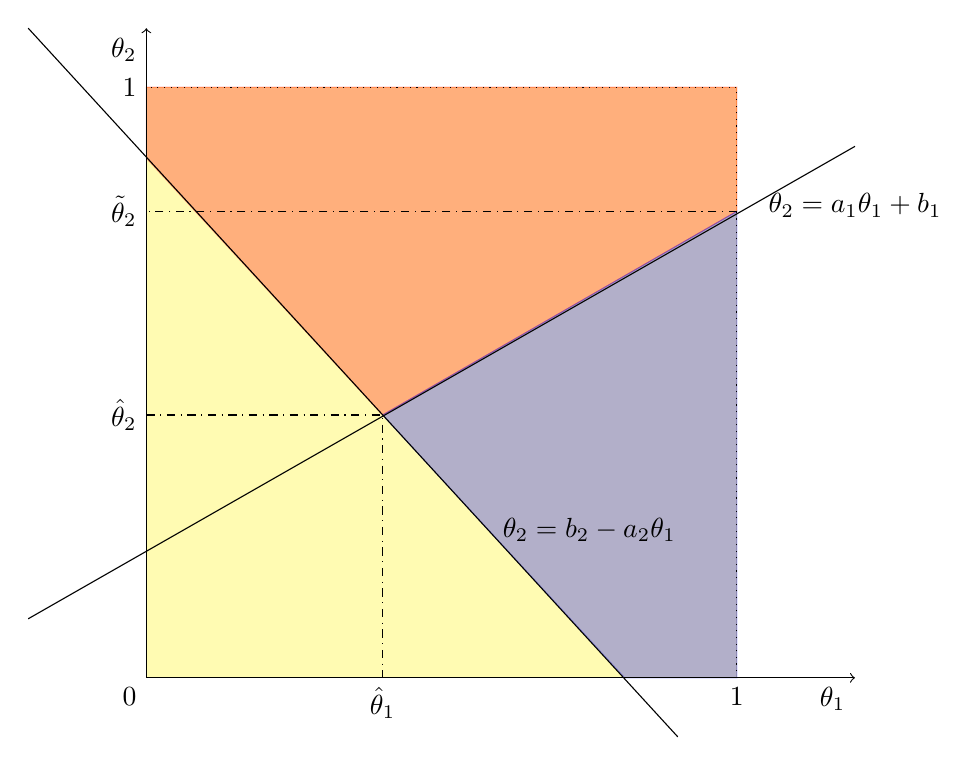
\begin{tikzpicture}[scale=7.5]
			%regions
			\filldraw[yellow, opacity=0.3] (0,0) -| (1,1) -| (0,0);
			\filldraw[red, opacity=0.3] (0,0.88) -- (0.4,0.445) -- (1,0.79) |- (0,1) -- (0,0.88);
			\filldraw[blue, opacity=0.3] (0.81,0) -- (0.4,0.445) -- (1,0.79) |- (0.81,0);
			
			% axes 
			\draw[->] (0,0) -- (1.2,0) node[below left]{$\theta_1$};
			\draw[->] (0,0) -- (0,1.1) node[below left]{$\theta_2$};
			\draw (0,0) node[below left]{$0$};
			\draw (0,1) node[left]{$1$};
			\draw (1,0) node[below]{$1$};
			
			% bounding box
			\draw[dotted] (1,0) |- (0,1);
			
			% two lines
			\draw (-0.2,0.1) -- (1.2,0.9);
			\draw (-0.2, 1.1) -- (0.9,-0.1);
			\draw (1.2,0.8) node {$\theta_2 = a_1 \theta_1 + b_1$};
			\draw (0.75,0.25) node {$\theta_2 = b_2 - a_2 \theta_1$};
			
			% special notation
			\draw[dashdotted] (1,0.79) -- +(-1,0) node[left]{$\tilde{\theta}_2$};
			\draw[dashdotted] (0,0.445) node[left]{$\hat{\theta}_2$} -| +(0.4,-0.445) node[below]{$\hat{\theta}_1$};
		\end{tikzpicture}
		\caption{an arbitrary allocation}
		\label{fig:2}
	\end{center}
\end{figure}

We will work with Figure \ref{fig:2}. Of course, there will be some things that are specific to the drawing, but the way we will solve the exercise should illustrate the general procedure for different figures.

Based on the figure, we construct the following allocation:
\begin{align*}
	k_1(\theta_1,\theta_2) &=
	\begin{cases}
		0 & \text{ if } \theta_2+a_2\theta_1\leq b_2\quad \text{ or }\quad \theta_2\geq b_1+a_1\theta_1\\
		1 & \text{otherwise}
	\end{cases}
	\\
	k_2(\theta_1,\theta_2) &=
	\begin{cases}
		0 & \text{ if } \theta_2+a_2\theta_1\leq b_2\quad \text{ or }\quad \theta_2\leq b_1+a_1\theta_1\\
		1 & \text{otherwise}
	\end{cases}
\end{align*}

We know that the allocation must be monotone for it to be implementable. However, it is very easy to check (just observe the drawing) that fixing the type of the other player, the probability of getting the good weakly increases with the player's type. Now we have to construct the transfers to implement this in dominant strategies. We will make use of the envelope representation of utility, mainly of the result that:
\begin{align} \label{transfer}
	t_i(\theta_i,\theta_{-i}) = \theta_i k_i(\theta_i,\theta_{-i}) - U_i(\underline{\theta}_{i}) - \int_{\underline{\theta}_{i}}^{\theta_i} k_{i} (u,\theta_{-i}) du
\end{align}
are the transfers that work.

Let's start with $t_1(\theta_1,\theta_2)$. Note that if $\theta_2>\tilde{\theta}_2$, then no matter what type player 1 announces, $k_1(\cdot,\theta_2)=0$. Hence, $t_1(\theta_1,\theta_2)=0$ for $\theta_2>\tilde{\theta}_2$. Consider now $\theta_2\in[\hat{\theta}_2,\tilde{\theta}_2]$. In that case, $k_1(\theta_1,\theta_2)=1$ if and only if $\theta_1\geq\frac{\theta_2-b_1}{a_1}$. Then for $\theta_2\in[\hat{\theta}_2,\tilde{\theta}_2]$:

\[t_1(\theta_1,\theta_2)=\left\{\begin{array}{cc} 0 & \quad\text{ if }\quad  \theta_1\leq\frac{\theta_2-b_1}{a_1}\\
	\frac{\theta_2-b_1}{a_1} & \quad\text{otherwise}\quad
	
\end{array}
\right.
\]
where the last part comes from using (\ref{transfer}) and noticing that $\underline{\theta}_1=\frac{\theta_2-b_1}{a_1}$ and setting $U_1(\underline{\theta}_1)=0$:
\begin{align*}
	t_1(\theta_1,\theta_2)=\theta_1-\int_{\frac{\theta_2-b_1}{a_1}}^{\theta_1}1 du=\frac{\theta_2-b_1}{a_1}
\end{align*}
Finally, consider $\theta_2\leq\hat{\theta}_2$. In that case, $k_1(\cdot,\theta_2)=0$ for $\theta_1\leq \frac{b_2-\theta_2}{a_2}=\underline{\theta}_1$. Then, in that case:

\[t_1(\theta_1,\theta_2)=\left\{\begin{array}{cc} 0 & \quad\text{ if }\quad  \theta_1\leq\frac{b_2-\theta_2}{a_2}\\
	\frac{b_2-\theta_2}{a_2} & \quad\text{otherwise}\quad
	
\end{array}
\right.
\]

Notice that, apart from Problem 3 saying it is the case, it is clear why the mechanism is DSIC: whether the player pays or not depends on his announcement, but not how much he pays. In this sense, it is like a SPA.

We can calculate the transfers for player 2 in a similar manner. Consider $\theta_1<\hat{\theta}_1$. Then, $k_2(\theta_1,\theta_2)=0$ if $\theta_2\leq b_2-a_2 \theta_1$. Then,

\[t_2(\theta_1,\theta_2)=\left\{\begin{array}{cc} 0 & \quad\text{ if }\quad  \theta_2\leq b_2-a_2 \theta_1\\
	b_2-a_2 \theta_1 & \quad\text{otherwise}\quad
	
\end{array}
\right.
\]
On the other hand, if $\theta_1\geq\hat{\theta}_1$, we have that $k_2(\theta_1,\theta_2)=0$ if $\theta_2\leq a_1\theta_1+b_1$. Then:
\[t_2(\theta_1,\theta_2)=\left\{\begin{array}{cc} 0 & \quad\text{ if }\quad  \theta_2\leq b_1+a_1 \theta_1\\
	b_1+a_1 \theta_1 & \quad\text{otherwise}\quad
	
\end{array}
\right.
\]



Now for the last part of the question: whether there exists a DSIC allocation rule that cannot be represented by a drawing described in the problem. The answer is yes, one example is as follows.
Consider the allocation depicted in Figure \ref{fig:3}, which is given by (the exact numbers do not matter):
\begin{align*}
	k(\theta_1,\theta_2) = \begin{cases}
		1 & \text{ if } \theta_1 \geq \max\{ 0.7 - \theta_2, \ 0.2 + \theta_2 \};
		\\
		2 & \text{ if } \theta_2 \geq \max\{ 0.7 - \theta_1, \ 0.2 + \theta_1 \};
		\\
		0 & \text{ otherwise.}
	\end{cases}
\end{align*}

This allocation is again monotone for each player ($k_i$ weakly increasing in $\theta_i$ given fixed $\theta_j$). We can construct the transfers that DSIC-implement it in the same way as we did in the main problem above (using \eqref{transfer}).

\begin{figure}
	\centering
	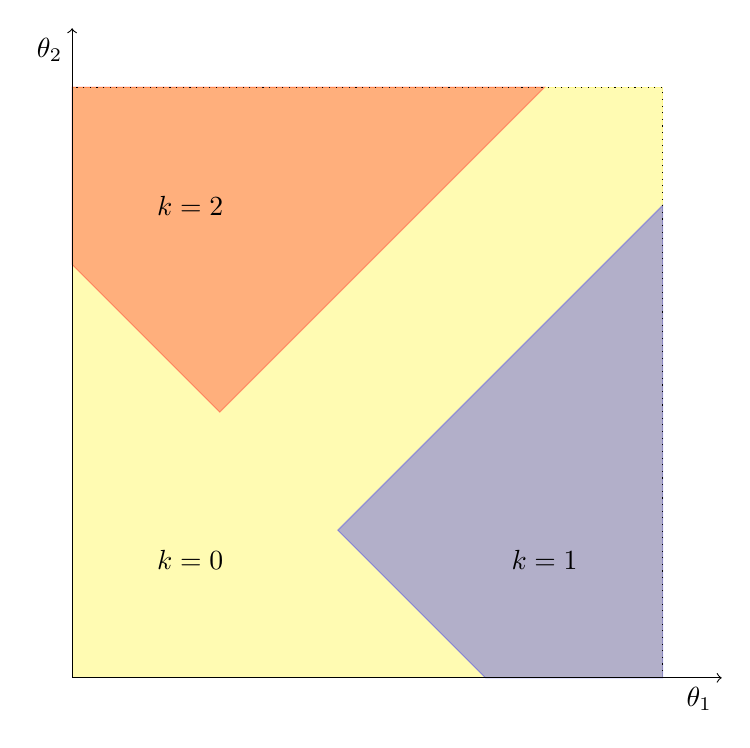
\begin{tikzpicture}[scale=7.5]
		\filldraw[yellow, opacity=0.3] (0,0) -| (1,1) -| (0,0);
		\filldraw[red, opacity=0.3] (0,0.7) -- (0.25,0.45) -- (0.8,1) -| (0,0.7);
		\filldraw[blue, opacity=0.3] (0.7,0) -- (0.45,0.25) -- (1,0.8) |- (0.7,0);
		
		\draw(0.2,0.2) node{$k=0$};
		\draw(0.2,0.8) node{$k=2$};
		\draw(0.8,0.2) node{$k=1$};
		
		% axes 
		\draw[->] (0,0) -- (1.1,0) node[below left]{$\theta_1$};
		\draw[->] (0,0) -- (0,1.1) node[below left]{$\theta_2$};
		
		% bounding box
		\draw[dotted] (1,0) |- (0,1);
	\end{tikzpicture}
	\caption{an even more arbitrary DSIC allocation} \label{fig:3}
\end{figure}

\fi



\section{Payoff equivalence in auctions}

Consider an auction for one item and $N$ bidders with valuations $\theta_i \sim i.i.d.U[0,1]$ and quasilinear preferences. Consider three different auction formats, in which all bidders submit bids simultaneously:
\begin{itemize}
	\item \emph{First-price sealed bid auction}, in which the highest bidder wins the item and pays their own bid. In such a format with $\theta_i \sim U[0,1]$, bidder $i$'s equilibrium bidding strategy is $b_i^{FPA} = \frac{N-1}{N} \theta_i$.
	\item \emph{Second-price sealed bid auction}, in which the highest bidder wins and pays the second-highest bid. In such a format, it is a weakly dominant strategy for bidder $i$ to bid their valuation: $b_i^{SPA} = \theta_i$.
	\item \emph{All-pay auction}, in which all bidders pay their bids, and the highest bidder wins the item. In such a format with $\theta_i \sim U[0,1]$, bidder $i$'s equilibrium bidding strategy is $b_i^{APA} = \frac{N-1}{N} \theta_i^N$.
\end{itemize}
Calculate the bidders' (interim) expected payoffs and the auctioneer's (ex ante) expected revenues under the three formats. Verify that they are the same across the three cases.

\emph{Bonus question:} verify that the bidding functions given for FPA and APA do indeed constitute an equilibrium.

\ifsolutions
\section*{Solution}

We use the following notation conventions, given some player $i$:
\begin{align*}
	%\bar{k}_i(\theta_i) &\equiv \mathbb{E}_{\theta_{-i}} \left[ k_i(\theta_i,\theta_{-i}) \right],
	%\\
	%\bar{t}_i(\theta_i) &\equiv \mathbb{E}_{\theta_{-i}} \left[ t_i(\theta_i,\theta_{-i}) \right],
	%\\
	\bar{U}_i(\theta_i) &\equiv \mathbb{E}_{\theta_{-i}} \left[ \theta_i \bar{k}_i(\theta_i) - \bar{t}_i(\theta_i) \right],
	\\
	\theta_{(2)} &\equiv \max_{j \in \{1,...,N\} \backslash \{i\}} \theta_j .
\end{align*}
(The $\theta_{(2)}$ is a somewhat weird notation, since its value depends on both the $i$'s identity and the type profile $\theta$, neither of which is reflected in the notation -- which should be more like $\theta_{(2),i}(\theta)$ or $\theta_{(2)}(\theta_{-i})$. Both of the latter options feel quite heavy though, hence we use simply $\theta_{(2)}$.)

Further, it will prove useful to derive the distribution of $\max_{i \in \{1,...,N\}} \theta_i$. Its cdf is given by $F_N(x)$ such that
\begin{equation} \label{eq:auc_Fmax}
\begin{aligned}
	F_{N}(x) 
	&= \mathbb{P} \left\{ \max_{i \in \{1,...,N\}} \theta_i \leq x \right\}
	\\
	&= \prod_{j \in \{1,...,N\}} \mathbb{P} \left\{ \theta_j \leq x \right\}
	\\
	&= x^N,
\end{aligned}
\end{equation}
where the second equality follows from the independence of players' valuations, and the final equality uses $\theta_j \sim U[0,1]$. The respective pdf is then given by $\phi_{N}(x) = Nx^{N-1}$.

\paragraph{FPA.} 
Given the proposed bidding strategy, the highest-valuation player wins the item. Bidder $i$'s interim expected payoff is
\begin{align*}
	\bar{U}_i(\theta_i) &= \mathbb{E}_{\theta_{-i}} \left[ \left( \theta_i - \frac{N-1}{N} \theta_i \right) \cdot \mathbb{I} \left\{ \theta_i > \theta_j, \forall j \neq i \right\} \right]
	\\
	&= \mathbb{E}_{\theta_{-i}} \left[ \frac{\theta_i}{N} \cdot \mathbb{I} \left\{ \theta_i > \theta_j, \forall j \neq i \right\} \right]
	\\
	&= \frac{\theta_i}{N} \cdot \mathbb{E}_{\theta_{-i}} \left[ \mathbb{I} \left\{ \theta_i > \theta_{(2)} \right\} \right]
\end{align*}
where the third inequality follows from the definition of $\theta_{(2)}$ and from $\frac{\theta_i}{N}$ being independent of $\theta_{-i}$. Then since $\theta_i$ is fixed, and the expectation of an indicator of an event is simply the probability of this event, we get
\begin{align*}
	\bar{U}_i(\theta_i) 
	&= \frac{\theta_i}{N} \cdot \mathbb{P} \left\{ \theta_{(2)} < \theta_i \right\}
	= \frac{\theta_i}{N} \cdot F_{N-1} (\theta_i)
	= \frac{\theta_i}{N} \cdot \theta_i^{N-1}
	= \frac{\theta_i^N}{N}.
\end{align*}
To show that the suggested strategy indeed constitutes an equilibrium, take some bidder $i$, suppose all other players bid according to $b_j(\theta_j) = \frac{N-1}{N} \theta_j$, and maximize $i$'s interim expected utility w.r.t. their bid $b_i$:
\begin{align*}
	\bar{U}_i(b_i,\theta_i) &= \mathbb{E}_{\theta_{-i}} \left[ \left( \theta_i - b_i \right) \cdot \mathbb{I} \left\{ b_i > \frac{N-1}{N} \theta_j, \forall j \neq i \right\} \right]
	\\
	&= (\theta_i - b_i) \cdot F_{N-1} \left(\frac{N b_i}{N-1} \right) = (\theta_i - b_i) \cdot \left(\frac{N b_i}{N-1} \right)^{N-1}.
\end{align*}
Taking the FOC of the maximization problem and solving it for $b_i$, we get
\begin{align*}
	\frac{d \bar{U}_i(b_i,\theta_i)}{db_i} 
	&= \left(\frac{N}{N-1} \right)^{N-1} \left[(N-1) \theta_i b_i^{N-2} - N b_i^{N-1} \right] = 0
	\\ \Rightarrow
	b_i^* &= \frac{N-1}{N} \theta_i,
\end{align*}
as conjectured.

Moving on to the designer's profit, 
\begin{align*}
	\mathbb{E}_\theta [R] = - \mathbb{E}_\theta[t_0(\theta)]
	&= \mathbb{E}_\theta \left[ \sum_{i=1}^N t_i(\theta) \right]
	\\
	&= \mathbb{E}_\theta \left[ \max_{i \in \{1,...,N\}} b_i(\theta_i) \right]
	\\
	&= \mathbb{E}_\theta \left[ \max_{i \in \{1,...,N\}} \frac{N-1}{N} \theta_i \right]
	\\
	&= \frac{N-1}{N} \mathbb{E}_\theta \left[ \max_{i \in \{1,...,N\}} \theta_i \right]
	\\
	&= \frac{N-1}{N} \int_0^1 x \phi_{N} (x) dx
	\\
	&= \frac{N-1}{N} \int_0^1 N x^N dx
	\\
	&= \frac{N-1}{N+1}.
\end{align*}
In the end, in FPA, $\bar{U}_i(\theta_i) = \frac{\theta_i^N}{N}$ and $\mathbb{E}_\theta [R] = 
\frac{N-1}{N+1}$.


\paragraph*{APA}
Following the same logic,
\begin{align*}
	\bar{U}_i(\theta_i) &= \mathbb{E}_{\theta_{-i}} \left[ \theta_i \cdot \mathbb{I} \left\{ \theta_i > \theta_j, \forall j \neq i \right\} - \frac{N-1}{N} \theta_i^N \right]
	\\
	&= \theta_i \cdot \theta_i^{N-1} - \frac{N-1}{N} \theta_i^N
	= \frac{\theta_i^N}{N}.
\end{align*}
In the second equality above, the first term is obtained using the exact same calculations as for FPA, and the second term lacks the expectation because it does not depend on $\theta_{-i}$.

To verify that the proposed strategy is optimal, proceed as in FPA:
\begin{align*}
	\bar{U}_i(b_i,\theta_i) &= \mathbb{E}_{\theta_{-i}} \left[ \theta_i \cdot \mathbb{I} \left\{ b_i > \frac{N-1}{N} \theta_j^N, \forall j \neq i \right\} - b_i \right]
	\\
	&= \theta_i F_{N-1} \left( \left( \frac{ N b_i}{N-1} \right)^\frac{1}{N} \right) - b_i
	\\
	&= \theta_i \left( \frac{ N b_i}{N-1} \right)^\frac{N-1}{N} - b_i
	\\ \Rightarrow
	\frac{d \bar{U}_i(b_i,\theta_i)}{db_i} 
	&= \theta_i \left( \frac{ N }{N-1} \right)^\frac{-1}{N} b_i^\frac{-1}{N} - 1 = 0
	\\ \Rightarrow
	b_i^* &= \frac{N-1}{N} \theta_i^N,
\end{align*}
as conjectured.

For the designer's expected revenue,
\begin{align*}
	\mathbb{E}_\theta [R]
	&= \mathbb{E}_\theta \left[ \sum_{i=1}^N t_i(\theta) \right]
	\\
	&= \mathbb{E}_\theta \left[ \sum_{i=1}^N \frac{N-1}{N} \theta_i^N \right]
	\\
	&= \sum_{i=1}^N \frac{N-1}{N} \mathbb{E}_{\theta_i} \left[ \theta_i^N \right]
	\\
	&= (N-1) \int_0^1 x^N dx
	\\
	&= \frac{N-1}{N+1}.
\end{align*}
The third inequality above splits the expectation of the sum into the sum of expectations (using the linearity of the expectation operator) and notices that the expectation of $\theta_i^N$ only depends on the realization of $\theta_i$, but not on any of the other $\theta_j$. The fourth equality collapses the sum (since all the expectations are equal, due to symmetric distribution of valuations) and rewrites the expectation explicitly (with the pdf of $\theta_i$ being $\phi(x)=1$ for $x \in [0,1]$).


\paragraph*{SPA}
Interim expected utility for the bidder:
\begin{align*}
	\bar{U}_i(\theta_i) &= \mathbb{E}_{\theta_{-i}} \left[ \left( \theta_i - \theta_{(2)} \right) \cdot \mathbb{I} \left\{ \theta_i > \theta_j, \forall j \neq i \right\} \right]
	\\
	&= \theta_i \cdot \theta_i^{N-1} - \mathbb{E}_{\theta_{-i}} \left[ \theta_{(2)} \cdot \mathbb{I} \left\{ \theta_i > \theta_j, \forall j \neq i \right\} \right]
	\\
	&= \theta_i^N - \mathbb{E}_{\theta_{(2)}} \left[ \theta_{(2)} \cdot \mathbb{I} \left\{ \theta_{(2)} < \theta_i \right\} \right]
	\\
	&= \theta_i^N - \int_0^1 \left[ x \cdot \mathbb{I} \left\{ x < \theta_i \right\} \right] (N-1)x^{N-2} dx
	\\
	&=\theta_i^N - (N-1) \int_0^{\theta_i} x^{N-1} dx
	\\
	&=\theta_i^N - \frac{N-1}{N} \theta_i^N = \frac{\theta_i^N}{N}.
\end{align*}
In the above, the second equality uses the same calculation as FPA for the first term. All other manipulations concern the second term. The third equality notices that out of all information about all $\theta_{-i}$, only $\theta_{(2)}$ is relevant. The fourth equality writes the expectation down explicitly, using the distribution obtained in \eqref{eq:auc_Fmax}. The remainder is just algebra.

The expected revenue of the designer is given by:
\begin{align*}
	\mathbb{E}_\theta [R]
	&= \mathbb{E}_\theta \left[ \sum_{i=1}^N t_i(\theta) \right]
	\\
	&= \mathbb{E}_\theta \left[ \theta_{(2)} \right].
\end{align*}
However, the meaning of $\theta_{(2)}$ is different here, which should ideally be reflected in the notation but isn't. In the previous cases, when we took $\theta_i$ as fixed and took expectation over $\theta_{-i}$, it was the case that simply $\theta_{(2)} = \max_{j \in \{1,...,N\} \backslash \{i\}} \theta_j$, i.e., it was the highest valuation among $N-1$ bidders. Now, though, we need to genuinely calculate the \emph{second-highest bid among $N$ bidders}. We can derive its pdf $\phi_{(2)}(x)$ as the probability, for any $x$, that exactly $N-2$ valuations are below $x$, one valuation is at $x$, and one valuation is above $x$. Since the latter two can belong to any bidder, there are a total of $N(N-1)$ permutations. In the end:
\begin{align*}
	\phi_{(2)}(x) &= N (N-1) \cdot x^{N-2} \cdot 1 \cdot (1-x)
	\\ \Rightarrow 
	\mathbb{E}_\theta [R] = \mathbb{E}_\theta \left[ \theta_{(2)} \right]
	&= \int_0^1 x N(N-1) x^{N-2} (1-x) dx
	\\
	&= N(N-1) \left[ \int_0^1 x^{N-1} dx - \int_0^1 x^N dx \right]
	\\
	&= N(N-1) \left[\frac{1}{N} - \frac{1}{N+1}\right]
	\\
	&= N(N-1) \frac{1}{N(N+1)} = \frac{N-1}{N+1}.
\end{align*}

Hence we see that bidders' interim expected utilities and the designer's expected revenue are indeed the same across all three formats.
%\mathbb{E}_{\theta_{-i}} \left[  \right]
\fi 



%%-----------------------------------------------------------------------------------------------------

\end{document}
